\documentclass[11pt, a4paperm, hidelinks]{article}
\usepackage[utf8]{inputenc}
\usepackage[T1]{fontenc}
\usepackage[english]{babel}
\usepackage{lmodern}


\usepackage[a4paper,top=3cm,bottom=3cm,left=3cm,right=3cm]{geometry}
\usepackage{chngcntr}

%package used to enumerate figures
\usepackage[labelfont=bf]{caption}

%hyperref for interactive PDF index
\usepackage[bookmarks, colorlinks, breaklinks]{hyperref}
\hypersetup{linkcolor=black, citecolor=black, filecolor=black, urlcolor=black}

%Package required to use special symbols
\usepackage{amsmath, amssymb}

%Package required to use figures
\usepackage{graphicx}
\usepackage{subfig}
\usepackage{placeins}
\usepackage{wrapfig}

%Include the bibliography in the table of contents
\usepackage{tocbibind}

%Package used to insert figures at the specified position
\usepackage{float}
\usepackage{longtable}

\usepackage{times}

%Our chapters must be called sections
\addto\captionsenglish{\renewcommand{\chaptername}{Section}}

%Header
\usepackage{fancyhdr}
\pagestyle{fancy}
\fancyhf{}
\rhead{Stefano Bagarin - Alessandra Pasini}
\lhead{Usability Evaluation Study 1: Inspection}
\rfoot{Page \thepage}

\begin{document}

	%Code for title page
	\begin{titlepage}
		\centering
		
\includegraphics[width=0.20\textwidth]{./assets/polimi-logo.png}\par

		{Politecnico di Milano \\ AA 2019/2020} \par
		\vspace{1.5cm}

		{Computer Science and Engineering}\par
		\Large{Hypermidia Applications}\par
		\vspace{1.0cm}

		{\LARGE \textbf{Usability Evaluation Study 1: Inspection} \par}
		\vspace{1.5cm}

		{\normalsize {\textbf{Stefano Bagarin}: mrt. 945159 -  stefano.bagarin@mail.polimi.it }\par}
		\vspace{0.2cm}
		{\normalsize{\textbf{Alessandra Pasini}: mtr. 920051 - alessandra.pasini@mail.polimi.it}\par}
		\vspace{1.0cm}
		
		{\normalsize {\textbf{Inspected website}: \url{https://www.visitmonterosa.com/}}\par}
		\vspace{0.2cm}
		{\normalsize {\textbf{Delivery Date}: }\par}
		\vfill

		% Bottom of the page
		{\large Document version: 1.0\par}
		{\large \today \par}
	\end{titlepage}

	%Make the table of contents
	\tableofcontents
	\clearpage


	%Abstract
	\section{Abstract}
	The aim of this document is to report the Inspection-based Usability Evaluation of \emph{Visit Monterosa} website which can be found at the following url \url{https://www.visitmonterosa.com/}. \\ TODO: The analysed website provides extensive
information about the Natural Park of Adamello – Brenta including descriptions of local history
and environment, activities and attractions available in the park paired with an interactive map of
tracks, initiatives organized by the park authorities and much more. The contents include an
analysis on through heuristic inspection of XX expert evaluators and an overall evaluation of the
product along with our conclusions. The Annex provides the individual scores of each inspector.


goal 1 : trovare esperienze e pronarle   “Searching information about experiences and opportunities”
goal 2 : prenotare vacanza 
goal 3 : avere informazioni sul monterosa
	\clearpage


	%Inspection Methods
	\section{Inspection Methods}

	\subsection{Overview}
	The inspection process started with the definition of both heuristics and score metrics, after a deep understanding of those concepts; then it went trough the choice of the main goals to have in mind while analyzing the website; the indivitual scoring and the final evaluation given by the average of individual ratings.\\
The following sections have the aim to highlight some of the steps taken during the inspection process and underline some foundamental concepts necessary to understand the final result.

	\subsection{Heuristic}
	The used heuristics can be divided into three cateogries depending on their final purposes and goals. Here is possible to find the groups definitions and the heuristics in each of them: \\ 
\\
\textbf{Navigation:} this batch has the aim to evaluate how easy is to move across the website and how easy and intuitive is to find contents following the websites paths.
	\begin{itemize}
		\item \textbf{Interaction consistency:} do pages of the same type have the same links and interaction capability?
		\item \textbf{Group navigation:} is it easy to navigate among group members and from a group introductory page to 				group members (and the other way around)?
		\item \textbf{Structural Navigation:} is it easy to navigate among the semantic components of a Topic?
		\item \textbf{Semantic Navigation:} is it easy to navigate from a Topic to a related one?
		\item \textbf{Landmarks:} are landmarks useful to reach the key parts of the web site?
	\end{itemize}
\textbf{Contents:} focuses on the quality of information and data provided by the site regardless the way they are presented. 
	\begin{itemize}
		\item \textbf{Information Overload:} is the information in a page too much or too little and does it fit the page layout?
		\item \textbf{Quality of Contents:} do the contents of the page include the informations that the user should expect 				there? In other words, is the content consistent.
	\end{itemize}
\textbf{Layout:} stresses the visual image of the website and its effectiveness in terms of expressivity and ergonomic functions. 
	\begin{itemize}
		\item \textbf{Text Layout:} is the text readable? Is font size appropriate?
		\item \textbf{Interaction Placeholder:} are textual or visual labels of interactive elements “expressive”? i.e., do they reflect 			the meaning of the interaction and its effects? Are they consistent?
		\item \textbf{Spatial Allocation:} is the on-screen allocation of contents and visual appropriate for their relevance? Are 				“semantically related” elements close and “semantically distant” element far away?
		\item \textbf{Consistency of Page Structure:} do pages of the same type have the same lay out (same visual properties of 			each component and similar lay-out organization of the various elements?) 
	\end{itemize}


	\subsection{Scoring Metrics}
	In order to evaluate every heuristic defined in the previous section, it has been choosen a scoring system with votes between 0 and 5. The following figure shows the meaning of each scores. 
\begin{figure}[h!]
	\centering
 	\begin{minipage}[b]{1\textwidth}
    		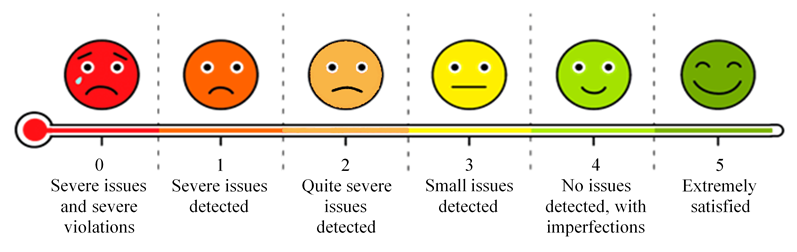
\includegraphics[width=\textwidth]{./assets/scoring.png}
	\end{minipage}
\end{figure}
\FloatBarrier

	\subsection{Goals}
	Before starting the process, the following goals have been defined to better inspect the website and to work in a more precise way.
\begin{itemize}
	\item \textbf{Goal 1:} Find experiences' information and book them
	\item \textbf{Goal 2:} Book an holiday
	\item \textbf{Goal 3:} Searching info about Monte Rosa

\end{itemize}


\subsection{Final Evaluation}
After an individual analysis of the website done by keeping in mind the goals previously selected, the final rating is estimated by doing the average of individual scores. Because of the fact that this is the most important and valuable part for the end user of this document it will be better analyzed in section 3 via tables, puntual comments and examples.


\subsection{Report}
This is the last step and corresponds to the writing of this document that explains the used procedure and the obtained results through scores and examples to support rating.
	\clearpage


	%Agreed scores on each individual heuristics
	\section{Agreed scores on each individual heuristics}

	\subsection{Navigation}
	\begin{figure}[h!]
	\centering
	\begin{minipage}[b]{1\textwidth}
    		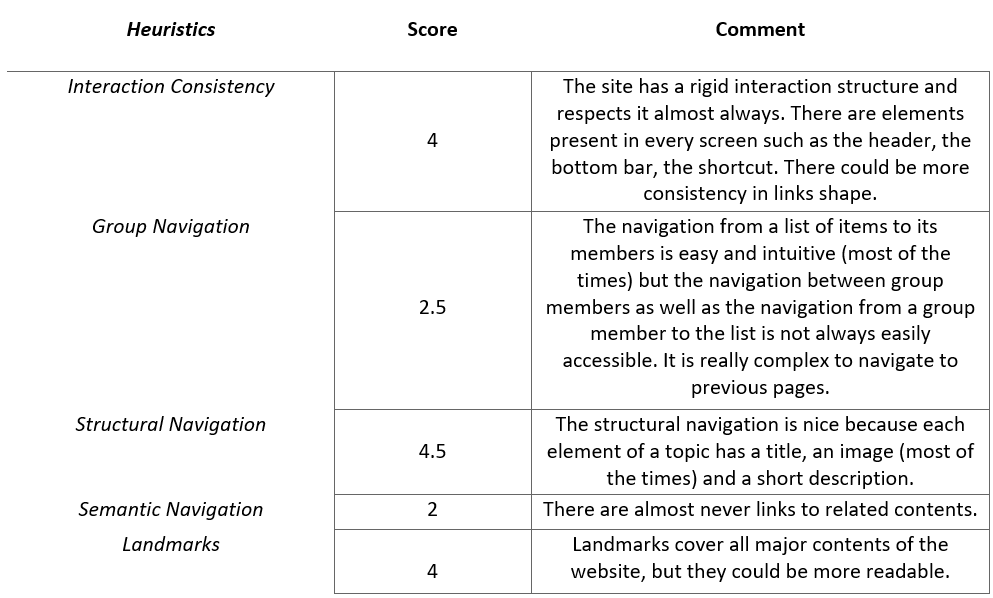
\includegraphics[width=\textwidth]{./assets/navigation-final.PNG}
	\end{minipage}
\end{figure}
\FloatBarrier
\subsubsection{Interaction Consistency}
This website has a pretty consistent choice of interaction. Every page shares the following elements:
\begin{itemize}
	\item \textbf{Header:} gives the possibility to change language, season and to access to the newsletter page (fig. 1) ;
	\item \textbf{Topbar:} allows a user to navigate between almost every website's page and content, it is the main navigation 		instrument (fig. 2); 
	\item \textbf{Leftbar:} allows a user to get important information such as weather, skilift 	situation, online skipass booking (fig. 		3);
	\item \textbf{Footer:} provides links to partners' websites, to its social network profiles and general informations such as 			contacts and privacy policies (fig. 4).
\end{itemize}  

\begin{figure}[h!]
	\centering
	\begin{minipage}[b]{0.7\textwidth}
    		
\includegraphics[width=\textwidth]{./assets/Interaction-header.png}
		\caption{Header}
	\end{minipage}
	\hfill
	\centering
	\begin{minipage}[b]{0.7\textwidth}
    		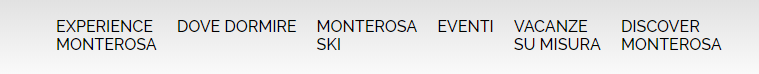
\includegraphics[width=\textwidth]{./assets/Interaction-topbar.png}
		\caption{Topbar}
	\end{minipage}
\end{figure}
\FloatBarrier

\begin{figure}[h!]
	\centering
	\begin{minipage}[b]{0.28\textwidth}
    		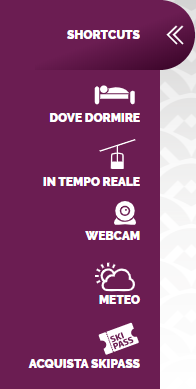
\includegraphics[width=\textwidth]{./assets/Interaction-leftbar.png}
		\caption{Leftbar}
	\end{minipage}
	\hfill
	\begin{minipage}[b]{0.65\textwidth}
    		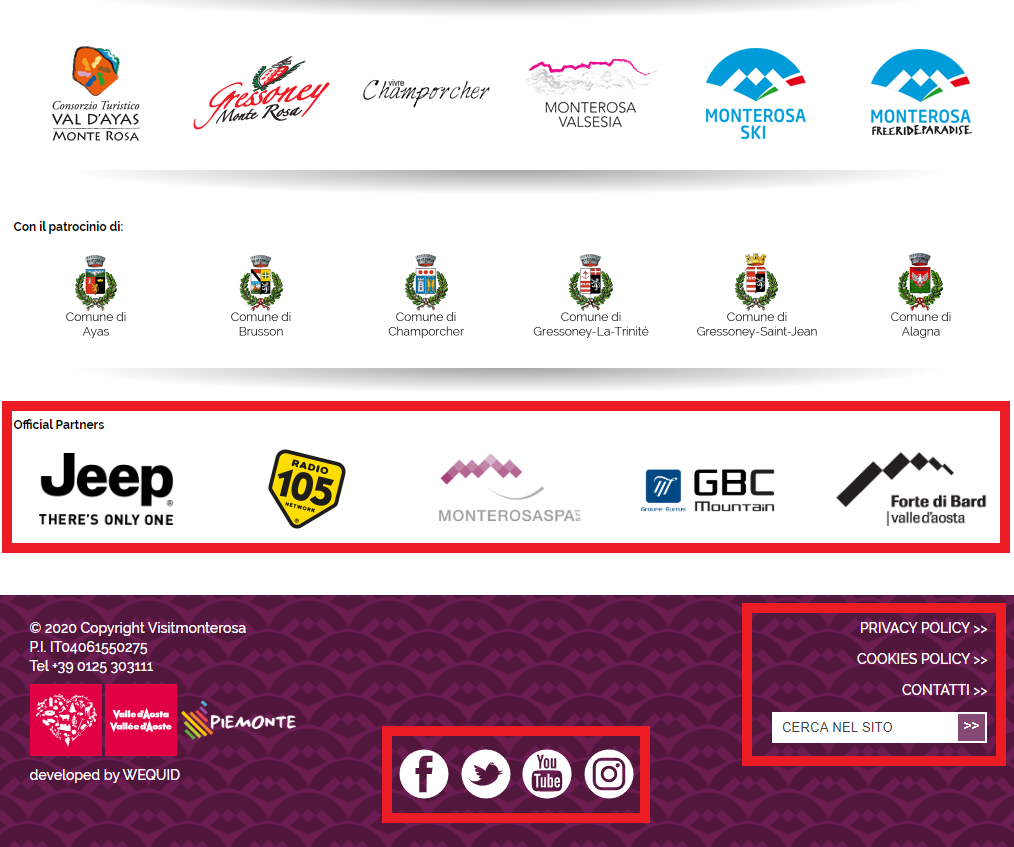
\includegraphics[width=\textwidth]{./assets/Interaction-bottom-bar.png}
		\caption{Footer}
	\end{minipage}
\end{figure}
\FloatBarrier

\subsubsection{Group Navigation}
\begin{wrapfigure}{r}{0.2\textwidth}
    	
\includegraphics[width=0.9\linewidth]{./assets/dropdown-menu.png}
	\caption{Dropdown Menù}
\end{wrapfigure} Thanks to the topbar (fig. 2) and the leftbar (fig. 3) a quick access is granted to almost all contents. Group navigation is also supported by topbar's dropdown menus (fig. 5), which contain the links to all main components of each group and helps the user to navigate between them. 

\subsubsection{Structural Navigation}
The various parts of a topic are organized in a list of items and each of them is represented by a title, a short description and almost always by an image; those elements makes the structural navigation realy intuitive.


\subsubsection{Semantic Navigation}
Semantic navigation is provided by links to the related pages that can be found for example in dropdown menu (fig. 5). Even though almost all contents can be accessed through the header, it is not possible to easily navigate between related contents because, except for some pages, similar contents aren't connect via a visible link. User can get confused also because there are also some links with an equivalent text label that bring to different pages with different contents. ????

\subsubsection{Landmarks}
Landmarks can be found into the header (fig. 1), the topbar (fig.2), the leftbar (fig. 3) and the footer (fig. 4). These elements do not change between different pages, but they could be more effective by adopting some graphic customization.

	\subsection{Content}
	\begin{figure}[h!]
	\centering
	\begin{minipage}[b]{1\textwidth}
    		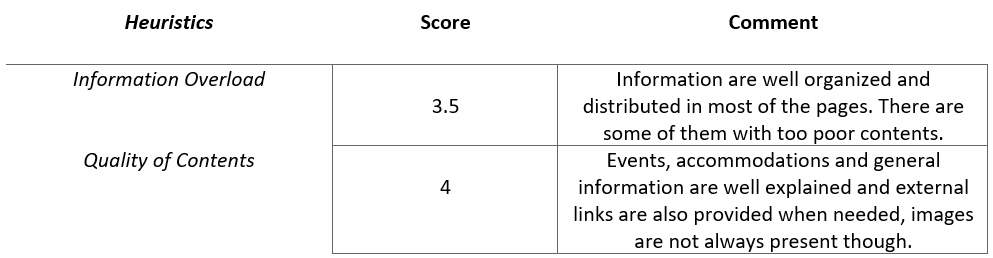
\includegraphics[width=\textwidth]{./assets/contents-final.PNG}
	\end{minipage}
\end{figure}
\FloatBarrier

\subsubsection{Information Overload}
Some pages do not contain any explanation of their contents except for the title. Sometimes the title is enough expressive, but the user experience loses clearness because of the poor text .
\FloatBarrier

\subsubsection{Quality of Contents}
Some graphical contents are missing, such as some images as in the accomodation element in figure 6.b.
\begin{figure}[h!]
	\subfloat[Accomodation card with complete information]{
		\begin{minipage}[b]{0.48\textwidth}
			\centering
			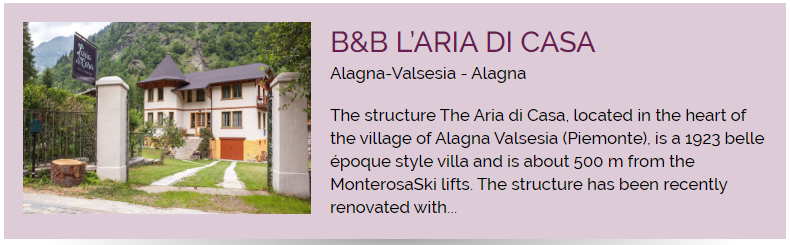
\includegraphics[width=\textwidth]{./assets/bnb-with-image.png}
		\end{minipage}}
		\hfill
	\subfloat[Accomodation card without complete information]{
		\begin{minipage}[b]{0.48\textwidth}
			\centering
			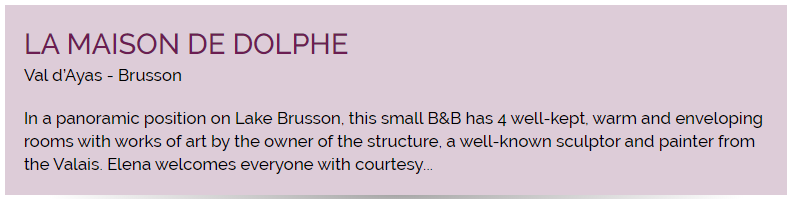
\includegraphics[width=\textwidth]{./assets/bnb-without-image.png}
		\end{minipage}}
		\hfill
	\caption{}
\end{figure}





	\subsection{Layout}
	\begin{figure}[h!]
	\centering
	\begin{minipage}[b]{1\textwidth}
    		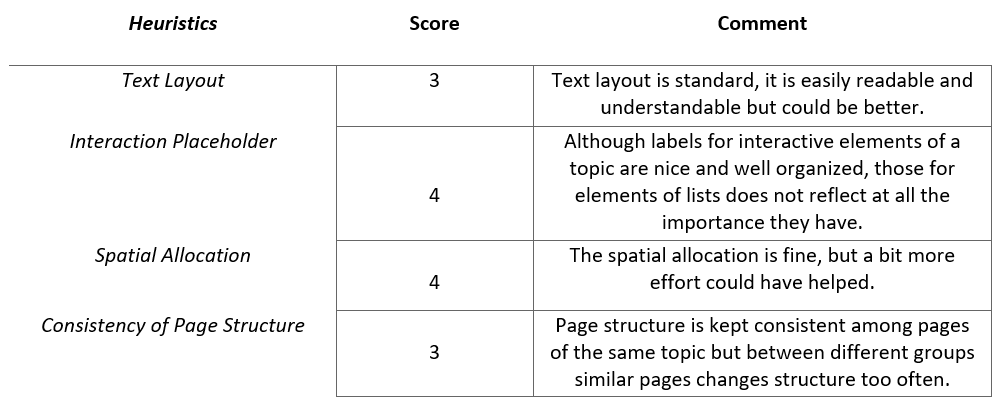
\includegraphics[width=\textwidth]{./assets/layout-final.PNG}
	\end{minipage}
\end{figure}
\FloatBarrier

\subsubsection{Text Layout}
Text layout is easily readable, but sometimes the font size is too small (10.5) and, with a longer text, it results more difficult to read it. Events and accomodations' cards could look tidier by adjusting image and text heights, by reducing titles dimension, justifing text, witout truncating it in the middle of a word and by giving it a bottom margin. Some cards, such as figure 6.a, respect the charateristics described above but most of them are shaped as figure 7.

\begin{figure}[h!]
	\centering
	\begin{minipage}[b]{1\textwidth}
    		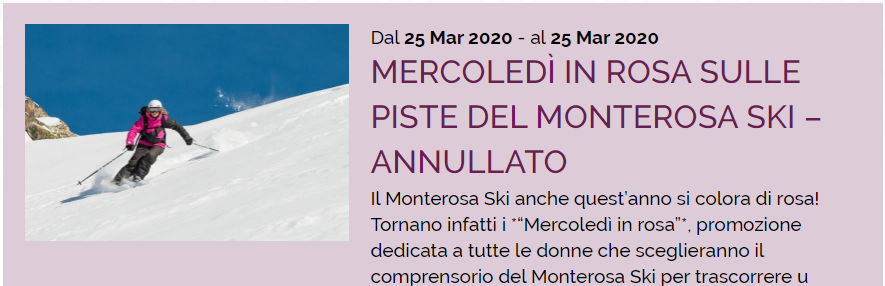
\includegraphics[width=\textwidth]{./assets/event.png}
		\caption{Untidy event card}
	\end{minipage}
\end{figure}
\FloatBarrier

\subsubsection{Interaction Placeholder}
Textual and visual labels are expressive almost in every case, a small neo is given by some textual links that aren't underlined and that, for this reason, seem to be normal and not clickable text. There are some inconcistency such as the fact that all header elements are link to general pages except for the textual label "Vacanze su misura" and the way in which filter buttons are labeled and shown. Some navigation buttons are expressive and consistent but could have a different layout (they could be bigger) in order to be more effective.

\subsubsection{Spatial Allocation}
Text and contents are well placed and reflect their relevance, but these elements could use pages' horizontal space in a better way.

\subsubsection{Concistency of Page Structure}
Pages belonging to the same groups or topics have similar layouts and they are consistent, but pages of different groups that are supposed to have same function aren't consistent and often have a different structure.
	\clearpage


	%Aggregated Results and Discussion
	\section{Aggregated Results and Conclusion}
	This section has the aim to aggregate all scores obtained in section 3 for each group, every value is computed as the average of heuristics' scores previously assigned and represents the overall evaluation about how navigation, contents and layout  is handled in "Visit Monterosa" website. Values are then approximeted by defect or by excess.

\subsubsection*{Navigation}
The navigation analysis is given by the five values corresponding to the 5 analyzed aspects: Interaction Consistency, Group Navigation, Structural Navigation, Semantic Navigation and Landmarks.\\
\textbf{Average: } ( 4 + 2.5 + 4.5 + 2 + 4) / 5 = 3.4  \emph{which can be approx to 3.5}\\
\begin{figure}[h!]
	\centering
	\begin{minipage}[b]{1\textwidth}
    		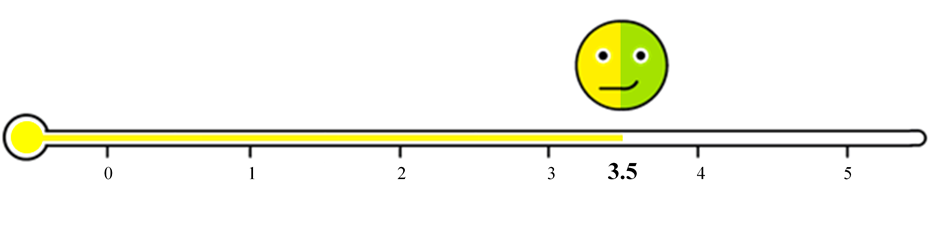
\includegraphics[width=1\textwidth]{./assets/layout-navigation-value.png}
	\end{minipage}
\end{figure}
\FloatBarrier

The mathematical average gives a 3.5 out of 5; this value underlines the fact that navigation is is pretty well handled, but with some issues that could be easily solved as reported in section 3.1.

\subsubsection*{Contents}
The overall evaluation about contents is given by the average of the 2 analyzed aspects.\\
\textbf{Average: } ( 3.5 + 4 ) / 2 = 3.75  \emph{which can be approx to 4}\\
\begin{figure}[h!]
	\centering
	\begin{minipage}[b]{1\textwidth}
    		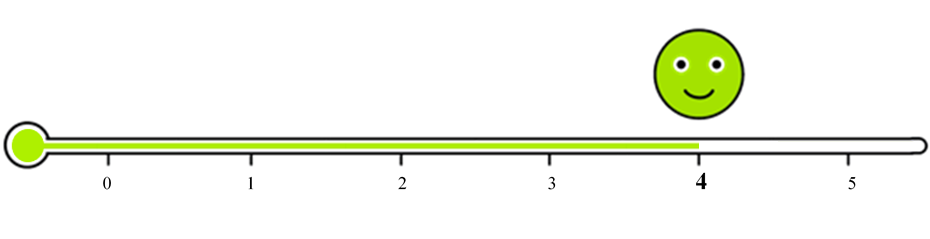
\includegraphics[width=1\textwidth]{./assets/contents-value.png}
	\end{minipage}
\end{figure}
\FloatBarrier

The mathematical average gives a 4 out of 5, a really high value. This evaluation is obtained because the website offers lots of information related to various topics and because they are quite well organized between pages. It could reach the maximum score by adding some little improvements as explained in section 3.2.

\subsubsection*{Layout}
For what concern the layout analysis, it has been done thanks to the evaluation of 4 foundamental aspects.\\
\textbf{Average: } ( 3 + 4 + 4 + 3 ) / 4 = 3.5 \\
\begin{figure}[h!]
	\centering
	\begin{minipage}[b]{1\textwidth}
    		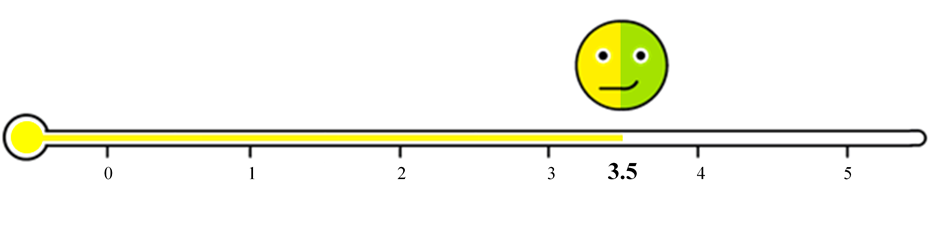
\includegraphics[width=1\textwidth]{./assets/layout-navigation-value.png}
	\end{minipage}
\end{figure}
\FloatBarrier

Also in this case the average gives a 3.5 out of 5; this value means that layout is pretty well done but could be improved more by adjusting some critical aspects such as Text Layout and the Concistency between pages.
	\clearpage

	\section{Conclusion}
	\clearpage

	%Appendix
	\appendix
	\section{Annex}
	The following tables are the ones upon which the final scores are obtained and they contain the individual ratings.

\begin{figure}[h!]
	\centering
 	 \begin{minipage}[b]{1\textwidth}
    		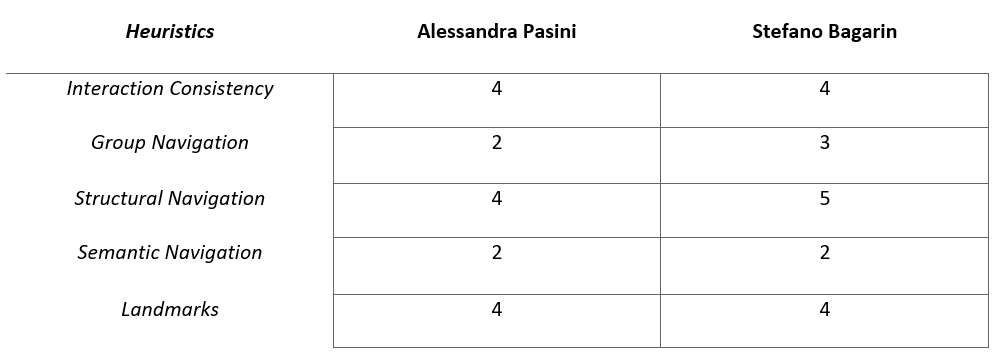
\includegraphics[width=\textwidth]{./assets/navigation.png}
    		\caption{Navigation}
  	\end{minipage}
	\hfill
	\vspace{1cm}
 	\begin{minipage}[b]{1\textwidth}
    		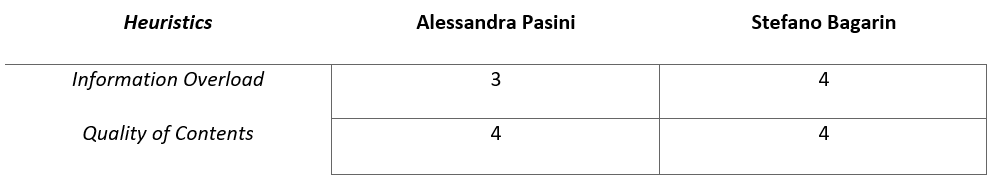
\includegraphics[width=\textwidth]{./assets/contents.png}
    		\caption{Contents}
	\end{minipage}
	\hfill
	\vspace{1cm}
	\begin{minipage}[b]{1\textwidth}
    		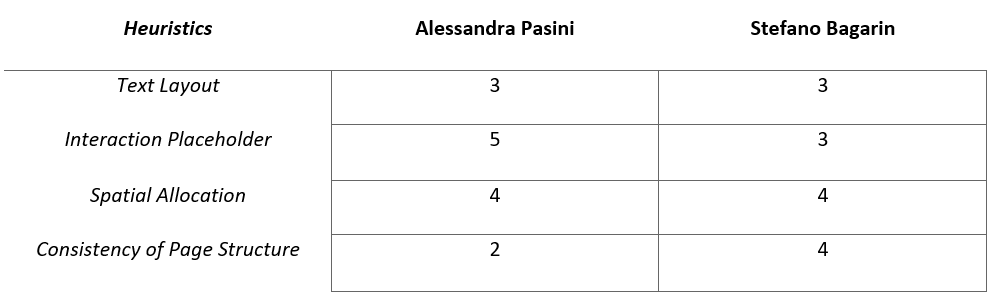
\includegraphics[width=\textwidth]{./assets/layout.png}
    		\caption{Layout}
	\end{minipage}
\end{figure}
\FloatBarrier



\end{document}
